% Pandoc LaTeX template — ACME arXiv paper
% Page 1: single-column title + abstract; body: two columns
\documentclass[11pt,a4paper]{article}

\usepackage{fontspec}
\IfFontExistsTF{Libertinus Serif}{%
  \setmainfont{Libertinus Serif}%
}{%
  \IfFontExistsTF{Times New Roman}{%
    \setmainfont{Times New Roman}%
  }{%
    \setmainfont{Latin Modern Roman}%
  }%
}
\IfFontExistsTF{Libertinus Sans}{%
  \setsansfont{Libertinus Sans}%
}{%
  \IfFontExistsTF{Helvetica Neue}{%
    \setsansfont{Helvetica Neue}%
  }{%
    \setsansfont{Latin Modern Sans}%
  }%
}
\setmonofont{Menlo}[Scale=0.85]

\usepackage{geometry}
\geometry{
  top=0.95in,
  bottom=0.95in,
  left=0.85in,
  right=0.85in,
  columnsep=0.28in
}

\usepackage[dvipsnames]{xcolor}
\usepackage{hyperref}
\usepackage{xurl}
\hypersetup{
  colorlinks=true,
  linkcolor=NavyBlue,
  urlcolor=NavyBlue,
  citecolor=NavyBlue,
  pdfauthor={Mohamed Kamil Bourouiba},
  pdftitle={ACME: Adaptive Cognitive Memory Engine}
}

\usepackage{setspace}
\setstretch{1.08}
\usepackage{parskip}
\setlength{\parskip}{0.42em plus 0.1em minus 0.08em}

\usepackage{titlesec}
\titleformat{\section}
  {\sffamily\large\bfseries}{\thesection.}{0.6em}{}
\titleformat{\subsection}
  {\sffamily\normalsize\bfseries}{\thesubsection}{0.6em}{}
\titleformat{\subsubsection}
  {\sffamily\normalsize\bfseries\itshape}{}{0em}{}
\titlespacing*{\section}{0pt}{2.4ex plus 1ex minus .2ex}{1.1ex plus .2ex}
\titlespacing*{\subsection}{0pt}{1.8ex plus .8ex minus .2ex}{0.8ex plus .2ex}
\titlespacing*{\subsubsection}{0pt}{1.4ex plus .6ex minus .2ex}{0.5ex plus .2ex}

\usepackage{booktabs}
\usepackage{array}
\usepackage{multirow}
\usepackage{calc}
\usepackage{colortbl}
\usepackage{siunitx}
\usepackage{makecell}
\usepackage{adjustbox}
\usepackage{needspace}
\usepackage{placeins}
\usepackage{tikz}
\usetikzlibrary{arrows.meta, positioning, shapes.geometric, fit, backgrounds, calc}
\usepackage{tcolorbox}
\tcbuselibrary{skins,breakable}

\renewcommand{\arraystretch}{1.35}
\setlength{\tabcolsep}{7pt}

\usepackage{microtype}
\usepackage{enumitem}
\setlist[itemize]{topsep=0.35em, itemsep=0.2em, parsep=0pt, leftmargin=1.4em}
\setlist[enumerate]{topsep=0.35em, itemsep=0.2em, parsep=0pt, leftmargin=1.4em}

\renewenvironment{abstract}{%
  \vspace{0.2em}%
  \begin{center}%
  \begin{minipage}{0.92\linewidth}%
  \textbf{\large\sffamily Abstract}\par\vspace{0.55em}%
  \itshape\small%
}{%
  \end{minipage}%
  \end{center}%
  \vspace{0.85em}%
}

\definecolor{keybg}{RGB}{245,248,252}
\definecolor{keyborder}{RGB}{0,82,120}
\definecolor{acmefigblue}{RGB}{0,82,120}
\definecolor{acmefiggray}{RGB}{100,110,125}
\definecolor{acmefiglight}{RGB}{235,242,248}
\definecolor{acmein}{RGB}{228,240,250}
\definecolor{acmemem}{RGB}{220,236,228}
\definecolor{acmereason}{RGB}{248,240,225}
\definecolor{acmefb}{RGB}{238,228,246}
\definecolor{acmerow}{RGB}{232,240,248}
\definecolor{bannerbg}{RGB}{241,245,249}

\newtcolorbox{keyfinding}{%
  enhanced,
  breakable,
  colback=keybg,
  colframe=white,
  boxrule=0pt,
  borderline west={2.5pt}{0pt}{keyborder},
  left=7pt, right=7pt, top=5pt, bottom=5pt,
  before skip=0.85em,
  after skip=0.95em,
  fontupper=\small
}
\newtcolorbox{contributions}{%
  enhanced,
  colback=keybg,
  colframe=keyborder!50,
  boxrule=0.35pt,
  arc=2pt,
  left=8pt, right=8pt, top=6pt, bottom=6pt,
  fonttitle=\sffamily\bfseries\small,
  title={Contributions},
  before skip=0.6em,
  after skip=0.85em,
  fontupper=\small
}
\newtcolorbox{metabox}{%
  enhanced,
  colback=bannerbg,
  colframe=keyborder!25,
  boxrule=0.3pt,
  arc=3pt,
  left=10pt, right=10pt, top=6pt, bottom=6pt,
  before skip=0pt,
  after skip=0pt
}
\newtcolorbox{bannerbox}{%
  enhanced,
  colback=bannerbg,
  colframe=keyborder!35,
  boxrule=0.35pt,
  arc=4pt,
  left=8pt, right=8pt, top=7pt, bottom=7pt,
  halign=center
}

\newcommand{\acmeTitleStrip}{%
  \begin{bannerbox}
    \small\sffamily\color{keyborder}
    LLM \textrightarrow\ Episodic Memory \textrightarrow\ Belief Engine \textrightarrow\
    Feedback Loop \textrightarrow\ Updated Beliefs
  \end{bannerbox}%
}

\providecommand{\tightlist}{%
  \setlength{\itemsep}{0pt}\setlength{\parskip}{0pt}}

\usepackage{caption}
\captionsetup{skip=0.55em, labelfont={bf,sf}, font=small}
\captionsetup[table]{position=above,skip=0.3em}

\usepackage{fvextra}
\DefineVerbatimEnvironment{Highlighting}{Verbatim}{breaklines,commandchars=\\\{\},xleftmargin=0.5em,fontsize=\footnotesize}

\clubpenalty=3000
\widowpenalty=3000
\displaywidowpenalty=3000

\newcommand{\acmeBackMatterBegin}{%
  \FloatBarrier
  \clearpage
  \onecolumn
}
\newcommand{\acmeReferencesBegin}{%
  \small
  \setlength{\parskip}{0.32em}%
  \setlength{\parindent}{-1.15em}%
  \setlength{\leftskip}{1.15em}%
}
\newcommand{\acmeReferencesEnd}{%
  \normalsize
  \setlength{\parindent}{0pt}%
  \setlength{\leftskip}{0pt}%
}

\sisetup{
  table-format=1.3,
  table-number-alignment=right,
  detect-weight=true,
  detect-family=true
}

\newcommand{\acmeTableHdr}{%
  \textbf{System} &
  {\textbf{Ret.}} &
  {\textbf{Gnd.}} &
  {\textbf{Fbk.}} &
  {\textbf{Bel.}} &
  {\textbf{Ovr.}} \\%
}

% Multi-line benchmark column headers (positioning tables)
\newcommand{\acmeBenchCols}{%
  \textbf{Capability} &
  \makecell[c]{\textbf{LongMem}\\\textbf{Eval}} &
  \makecell[c]{\textbf{MemAgent}\\\textbf{Bench}} &
  \makecell[c]{\textbf{Reflection}\\\textbf{Bench}} &
  \makecell[c]{\textbf{Mem}\\\textbf{Bench}} &
  \makecell[c]{\textbf{Memory}\\\textbf{Bench}} \\%
}
\newcommand{\acmeBenchColsProp}{%
  \textbf{Property} &
  \makecell[c]{\textbf{LongMem}\\\textbf{Eval}} &
  \makecell[c]{\textbf{MemAgent}\\\textbf{Bench}} &
  \makecell[c]{\textbf{Reflection}\\\textbf{Bench}} &
  \makecell[c]{\textbf{Mem}\\\textbf{Bench}} &
  \makecell[c]{\textbf{Memory}\\\textbf{Bench}} \\%
}


$if(highlighting-macros)$
$highlighting-macros$
$endif$

% Pandoc's snugshade code blocks ignore column width in twocolumn mode.
\DefineVerbatimEnvironment{Highlighting}{Verbatim}{%
  breaklines,breakanywhere=true,commandchars=\\\{\},%
  xleftmargin=0pt,xrightmargin=0pt,fontsize=\scriptsize}
\renewenvironment{Shaded}{%
  \begin{tcolorbox}[%
    enhanced,breakable,%
    colback=shadecolor,colframe=shadecolor,boxrule=0pt,%
    left=4pt,right=4pt,top=4pt,bottom=4pt,arc=2pt,%
    width=\linewidth,before skip=0.45em,after skip=0.55em]%
}{%
  \end{tcolorbox}%
}

\newcommand{\papertagline}{A production-tested cognitive memory substrate for belief lifecycle management in LLM agents.}

\begin{document}

% Styled result tables — column-safe in twocolumn layout

% Two-column table (fits one column width)
\newcommand{\acmeTableBlockCol}[2]{%
  \par\vspace{0.45em}%
  \noindent
  \begin{center}
    \footnotesize
    \captionof{table}{#1}%
    \setlength{\tabcolsep}{3.5pt}%
    \renewcommand{\arraystretch}{1.22}%
    \resizebox{\dimexpr\columnwidth-1pt\relax}{!}{%
      #2%
    }%
  \end{center}
  \par\vspace{0.65em}%
}

% Full-width table (spans both columns)
\newcommand{\acmeTableBlockWide}[2]{%
  \begin{table*}[t]
    \centering
    \scriptsize
    \setlength{\tabcolsep}{4pt}%
    \renewcommand{\arraystretch}{1.25}%
    \caption{#1}%
    #2%
  \end{table*}%
}

\newcommand{\acmeTableMetrics}{%
  \acmeTableBlockCol{MemoryBench v3.1 metrics.}{%
    \begin{tabular}{@{}>{\raggedright\arraybackslash}p{0.32\columnwidth}p{0.60\columnwidth}@{}}
      \toprule
      \textbf{Metric} & \textbf{Description} \\
      \midrule
      Retention & Concept coverage (synonyms accepted) \\
      Groundedness & Answer supported by ingested episodes \\
      Feedback correction & Belief adjustment after contradictions \\
      Belief quality & Mean CRS across tracked beliefs \\
      \bottomrule
    \end{tabular}%
  }%
}

\newcommand{\acmeTableSetup}{%
  \acmeTableBlockCol{Experimental configuration (Azure production).}{%
    \begin{tabular}{@{}>{\raggedright\arraybackslash}p{0.30\columnwidth}p{0.62\columnwidth}@{}}
      \toprule
      \textbf{Component} & \textbf{Configuration} \\
      \midrule
      LLM & Azure OpenAI GPT-4.1 \\
      Embeddings & \texttt{text-embedding-3-small}, 256D \\
      Database & Postgres Flexible + pgvector \\
      Graph & Neo4j 5.x on Container Apps \\
      Judge & Same deployment as extractor/reasoner \\
      Reproducibility & \texttt{/benchmark/memorybench},\\
      & async compare \\
      \bottomrule
    \end{tabular}%
  }%
}

\newcommand{\acmeTablePositioningCapabilities}{%
  \acmeTableBlockWide{Benchmark positioning --- evaluation capabilities (Table~1a).}{%
    \begin{tabular}{@{}>{\raggedright\arraybackslash}p{0.22\textwidth} *{5}{>{\centering\arraybackslash}p{0.13\textwidth}}@{}}
      \toprule
      \acmeBenchCols
      \midrule
      Long-horizon / multi-session & Yes & Yes & Partial & Yes & Yes \\
      Knowledge update & Yes & Yes & Partial & Partial & Yes \\
      Feedback / belief revision & No & Partial & Yes & Partial & \textbf{Scored} \\
      Hallucination / abstention & Yes & Partial & Partial & Partial & Yes \\
      \bottomrule
    \end{tabular}%
  }%
}

\newcommand{\acmeTablePositioningInfra}{%
  \acmeTableBlockWide{Benchmark positioning --- infrastructure and belief metrics (Table~1b).}{%
    \begin{tabular}{@{}>{\raggedright\arraybackslash}p{0.22\textwidth} *{5}{>{\centering\arraybackslash}p{0.13\textwidth}}@{}}
      \toprule
      \acmeBenchColsProp
      \midrule
      Per-scenario sandbox & No & Partial & Yes & Yes & \textbf{Yes} \\
      Contrarian verification & No & No & Partial & No & \textbf{Yes} \\
      Belief quality (CRS) & No & No & No & Partial & \textbf{Yes} \\
      Production API + persisted runs & No & No & No & No & \textbf{Yes} \\
      \bottomrule
    \end{tabular}%
  }%
}

\newcommand{\acmeTablePositioning}{%
  \acmeTablePositioningCapabilities
  \acmeTablePositioningInfra
  \FloatBarrier
}

\newcommand{\acmeScoreTable}[2]{%
  \acmeTableBlockCol{#1}{%
    \begin{tabular}{@{}l *{5}{S[table-format=1.3]}@{}}
      \toprule
      \acmeTableHdr
      \midrule
      #2%
      \bottomrule
    \end{tabular}%
  }%
}

\newcommand{\acmeTableMain}{%
  \acmeScoreTable{Primary benchmark (GPT-4.1, 13 scenarios, job \texttt{3b31e5e3}). Ret.=Retention, Gnd.=Groundedness, Fbk.=Feedback, Bel.=Belief quality, Ovr.=Overall.}{%
      \rowcolor{acmerow}
      \textbf{ACME} & \textbf{1.000} & \textbf{1.000} & \textbf{1.000} & \textbf{0.700} & \textbf{0.925} \\
      RAG-like & 0.969 & 0.977 & {---} & {---} & 0.487 \\
      MemGPT-insp. & 0.977 & 0.969 & {---} & {---} & 0.487 \\
      LangGraph-sty. & 0.900 & 0.977 & {---} & {---} & 0.469 \\%
  }%
}

\newcommand{\acmeTableMini}{%
  \acmeScoreTable{Model sensitivity --- GPT-4.1-mini (job \texttt{107d02c0}).}{%
      \rowcolor{acmerow}
      \textbf{ACME} & \textbf{0.892} & \textbf{0.838} & \textbf{1.000} & \textbf{0.700} & \textbf{0.858} \\
      RAG-like & 0.908 & 0.985 & {---} & {---} & 0.473 \\
      MemGPT-insp. & 0.915 & 1.000 & {---} & {---} & 0.479 \\
      LangGraph-sty. & 0.854 & 0.862 & {---} & {---} & 0.429 \\%
  }%
}

\newcommand{\acmeTableGptFiveFour}{%
  \acmeScoreTable{Model sensitivity --- GPT-5.4 (job \texttt{eb68f028}).}{%
      \rowcolor{acmerow}
      \textbf{ACME} & \textbf{0.952} & \textbf{0.839} & \textbf{1.000} & \textbf{0.701} & \textbf{0.873} \\
      RAG-like & 0.964 & 0.931 & {---} & {---} & 0.474 \\
      MemGPT-insp. & 0.975 & 0.939 & {---} & {---} & 0.478 \\
      LangGraph-sty. & 0.973 & 0.950 & {---} & {---} & 0.481 \\%
  }%
}

\newcommand{\acmeTableLongMemEvalProtocol}{%
  \acmeTableBlockWide{LongMemEval oracle protocol (industry benchmark [35]).}{%
    \begin{tabular}{@{}>{\raggedright\arraybackslash}p{0.22\textwidth} p{0.68\textwidth}@{}}
      \toprule
      \textbf{Component} & \textbf{Configuration} \\
      \midrule
      Dataset & \texttt{longmemeval\_oracle.json} (500 Q, evidence sessions) \\
      Ingest & ACME orchestrator / RAG-like / MemGPT-inspired on identical haystacks \\
      Scoring & Official type-specific yes/no judge (reference \texttt{evaluate\_qa.py}) \\
      Metrics & Overall accuracy + per \texttt{question\_type} breakdown \\
      Reproduce & \texttt{scripts/run\_longmemeval.py} (see \texttt{docs/LONGMEMEVAL.md}) \\
      \bottomrule
    \end{tabular}%
  }%
}

\newcommand{\acmeTableLongMemEvalKU}{%
  \acmeTableBlockWide{LongMemEval \texttt{knowledge-update} subset (78 Q, oracle, GPT-4.1, June 2026).}{%
    \resizebox{\dimexpr\textwidth-4pt\relax}{!}{%
    \begin{tabular}{@{}l *{3}{S[table-format=1.3]}@{}}
      \toprule
      \textbf{System} &
      {\textbf{Overall}} &
      {\textbf{KU}} &
      {\textbf{Abst.}} \\
      \midrule
      \rowcolor{acmerow}
      \textbf{ACME (transcript-first)} & \textbf{0.897} & \textbf{0.931} & 0.500 \\
      MemGPT-insp. & 0.872 & 0.903 & 0.500 \\
      RAG-like & 0.859 & 0.875 & 0.667 \\
      \bottomrule
    \end{tabular}%
    }%
  }%
}

\newcommand{\acmeTableLongMemEvalFull}{%
  \acmeTableBlockWide{LongMemEval oracle full split (500 Q, GPT-4.1, June 2026).}{%
    \resizebox{\dimexpr\textwidth-4pt\relax}{!}{%
    \begin{tabular}{@{}l *{7}{S[table-format=1.3]}@{}}
      \toprule
      \textbf{Sys.} &
      {\textbf{All}} &
      {\textbf{KU}} &
      {\textbf{Multi}} &
      {\textbf{Temp.}} &
      {\textbf{SS-U}} &
      {\textbf{SS-A}} &
      {\textbf{SS-P}} \\
      \midrule
      \rowcolor{acmerow}
      \textbf{ACME} & \textbf{0.876} & \textbf{0.944} & \textbf{0.793} & \textbf{0.803} & \textbf{1.000} & \textbf{1.000} & \textbf{0.900} \\
      MemGPT-insp. & 0.786 & 0.861 & 0.793 & 0.630 & 1.000 & 0.982 & 0.600 \\
      RAG-like & 0.776 & 0.875 & 0.793 & 0.622 & 1.000 & 0.964 & 0.467 \\
      \bottomrule
    \end{tabular}%
    }%
  }%
}

\newcommand{\acmeTableAblations}{%
  \acmeTableBlockWide{Component ablations (ACME-only, MemoryBench v3.1, GPT-4.1).}{%
    \resizebox{\dimexpr\textwidth-4pt\relax}{!}{%
    \begin{tabular}{@{}l *{6}{S[table-format=1.3]}@{}}
      \toprule
      \textbf{Configuration} &
      {\textbf{Ovr.}} &
      {\textbf{Ret.}} &
      {\textbf{Gnd.}} &
      {\textbf{Fbk.}} &
      {\textbf{Bel.}} &
      {$\Delta$} \\
      \midrule
      \rowcolor{acmerow}
      \textbf{Full ACME} & \textbf{0.925} & \textbf{1.000} & \textbf{1.000} & \textbf{1.000} & \textbf{0.700} & {---} \\
      No contrarian & 0.923 & 1.000 & 0.993 & 1.000 & 0.700 & -0.002 \\
      No belief sync & 0.731 & 0.996 & 1.000 & 0.929 & 0.000 & -0.194 \\
      No vector retrieval & 0.923 & 0.993 & 1.000 & 1.000 & 0.700 & -0.002 \\
      \bottomrule
    \end{tabular}%
    }%
  }%
}

% ACME TikZ figures

\tikzset{
  acmebox/.style={
    draw=acmefigblue!70,
    rounded corners=4pt,
    line width=0.55pt,
    align=center,
    font=\small\sffamily,
    inner sep=5pt,
    minimum width=3.35in,
    minimum height=0.52in
  },
  acmeboxin/.style={acmebox, fill=acmein},
  acmeboxmem/.style={acmebox, fill=acmemem},
  acmeboxreason/.style={acmebox, fill=acmereason},
  acmeboxfb/.style={acmebox, fill=acmefb},
  acmearrow/.style={-{Stealth[length=2.2mm]}, line width=0.65pt, draw=acmefigblue!80},
  acmeloop/.style={-{Stealth[length=2mm]}, line width=0.55pt, draw=acmefiggray, dashed}
}

\newcommand{\acmeFigureLoop}{%
  \begin{figure*}[t]
    \centering
    \begin{tikzpicture}[
      node distance=0.42in,
      every node/.style={transform shape}
    ]
      \node[acmeboxin] (user) {User / Environment};
      \node[acmeboxin, below=of user] (extract) {LLM Extraction};
      \node[acmeboxmem, below=of extract] (store) {Episodic Store + Semantic Graph};
      \node[acmeboxreason, below=of store] (belief) {Belief Engine};
      \node[acmeboxreason, below=of belief] (retrieve) {Hybrid Retrieval + Contrarian Verification};
      \node[acmeboxin, below=of retrieve] (answer) {Answer / Prediction};
      \node[acmeboxfb, below=of answer] (feedback) {Feedback + Outcome Validation};

      \draw[acmearrow] (user) -- (extract);
      \draw[acmearrow] (extract) -- (store);
      \draw[acmearrow] (store) -- (belief);
      \draw[acmearrow] (belief) -- (retrieve);
      \draw[acmearrow] (retrieve) -- (answer);
      \draw[acmearrow] (answer) -- (feedback);

      \draw[acmeloop] (feedback.east) -- ++(0.55in,0) |- node[pos=0.22, right, font=\scriptsize\sffamily, align=left] {Belief Update /\\Demotion /\\Consolidation} (belief.east);

      \begin{scope}[on background layer]
        \node[draw=acmefigblue!25, rounded corners=5pt, inner sep=6pt, fit=(user)(extract), label={[font=\scriptsize\sffamily\color{acmefiggray}]above left:Input / output}] {};
        \node[draw=acmefigblue!25, rounded corners=5pt, inner sep=6pt, fit=(store), label={[font=\scriptsize\sffamily\color{acmefiggray}]above left:Memory stores}] {};
        \node[draw=acmefigblue!25, rounded corners=5pt, inner sep=6pt, fit=(belief)(retrieve), label={[font=\scriptsize\sffamily\color{acmefiggray}]above left:Reasoning}] {};
        \node[draw=acmefigblue!25, rounded corners=5pt, inner sep=6pt, fit=(feedback), label={[font=\scriptsize\sffamily\color{acmefiggray}]above left:Feedback / update}] {};
      \end{scope}
    \end{tikzpicture}
    \caption{ACME cognitive loop: extraction, hybrid memory, belief governance, and closed-loop correction.}
    \label{fig:acme-loop}
  \end{figure*}%
}

\newcommand{\acmeFigureBelief}{%
  \begin{figure}[t]
    \centering
    \begin{tikzpicture}[
      node distance=0.24in and 0.08in,
      every node/.style={transform shape},
      scale=0.92, transform shape
    ]
      \node[acmeboxreason, minimum width=0.68in, minimum height=0.44in, font=\scriptsize\sffamily] (obs) {Observation};
      \node[acmeboxreason, right=of obs, minimum width=0.64in] (inf) {Inference};
      \node[acmeboxreason, right=of inf, minimum width=0.72in] (hyp) {Hypothesis};
      \node[acmeboxreason, right=of hyp, minimum width=0.58in] (bel) {Belief};

      \draw[acmearrow] (obs) -- (inf);
      \draw[acmearrow] (inf) -- (hyp);
      \draw[acmearrow] (hyp) -- (bel);

      \node[font=\scriptsize\sffamily\color{acmefiggray}, above=0.06in of hyp] {evidence accumulation / CRS increase};

      \node[acmeboxfb, below=0.48in of bel, minimum width=0.78in, minimum height=0.42in, font=\scriptsize\sffamily] (chal) {Challenged};
      \node[acmeboxfb, below=of chal, minimum width=0.95in, minimum height=0.42in] (dep) {Deprecated / Archived};

      \draw[acmearrow] (bel) -- (chal);
      \draw[acmearrow] (chal) -- (dep);

      \node[font=\scriptsize\sffamily\color{acmefiggray}, below=0.05in of chal] {contradiction / failed prediction};
    \end{tikzpicture}
    \caption{Belief lifecycle: promotion along evidence accumulation and demotion under contradiction.}
    \label{fig:belief-lifecycle}
  \end{figure}%
}

\newcommand{\acmeResultSummary}{%
  \begin{figure*}[t]
    \centering
    \small\sffamily
    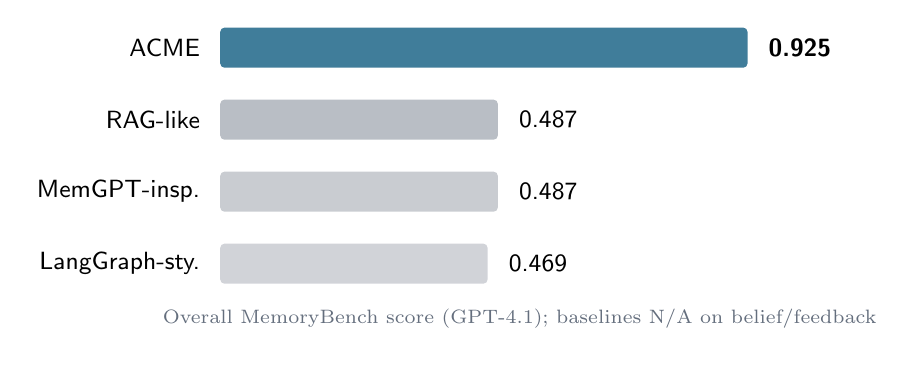
\begin{tikzpicture}[
      x=1in, y=0.36in,
      bar/.style={rounded corners=1.5pt, minimum height=0.20in, inner sep=0pt, anchor=west},
      lbl/.style={anchor=east, font=\small\sffamily},
      val/.style={anchor=west, font=\small\sffamily}
    ]
      \def\barscale{2.85}
      \node[lbl] at (0,3) {ACME};
      \node[bar, fill=acmefigblue!75, minimum width={0.925*\barscale in}] at (0.05,3) {};
      \node[val] at ($(0.05,3)+(0.925*\barscale in,0)+(0.06,0)$) {\textbf{0.925}};

      \node[lbl] at (0,2) {RAG-like};
      \node[bar, fill=acmefiggray!45, minimum width={0.487*\barscale in}] at (0.05,2) {};
      \node[val] at ($(0.05,2)+(0.487*\barscale in,0)+(0.06,0)$) {0.487};

      \node[lbl] at (0,1) {MemGPT-insp.};
      \node[bar, fill=acmefiggray!35, minimum width={0.487*\barscale in}] at (0.05,1) {};
      \node[val] at ($(0.05,1)+(0.487*\barscale in,0)+(0.06,0)$) {0.487};

      \node[lbl] at (0,0) {LangGraph-sty.};
      \node[bar, fill=acmefiggray!30, minimum width={0.469*\barscale in}] at (0.05,0) {};
      \node[val] at ($(0.05,0)+(0.469*\barscale in,0)+(0.06,0)$) {0.469};

      \node[font=\scriptsize\color{acmefiggray}, anchor=north] at (1.55,-0.5) {Overall MemoryBench score (GPT-4.1); baselines N/A on belief/feedback};
    \end{tikzpicture}
    \caption{Result summary: ACME leads primarily on feedback and belief-quality dimensions unavailable to baselines.}
    \label{fig:result-summary}
  \end{figure*}%
}


% --- Page 1: title + abstract (single column) ---
\begin{center}
  \vspace*{0.12in}
  {\sffamily\fontsize{24}{29}\selectfont\bfseries
   ACME: Adaptive Cognitive Memory Engine\par}
  \vspace{0.85em}
  {\sffamily\Large
   Externalizing Belief, Memory, and Learning from LLM Weights\par}
  \vspace{1.1em}
  {\normalsize\itshape\papertagline\par}
  \vspace{1.15em}
  {\normalsize Mohamed Kamil Bourouiba\par}
  \vspace{0.35em}
  {\footnotesize\copyright{} 2026 Mohamed Kamil Bourouiba. All rights reserved.\par}
  \vspace{0.45em}
  {\small arXiv preprint draft v1.2 --- June 2026\par}
  \vspace{0.85em}
  \acmeTitleStrip
  \vspace{0.65em}
  \begin{metabox}
    \begin{minipage}{0.88\linewidth}
      \footnotesize\sffamily\color{acmefiggray}
      \textbf{Code:} \url{https://github.com/KamilBourouiba/ACME} (tag \texttt{v0.1.1-arxiv})\\
      \textbf{Project site:} \url{https://kamilbourouiba.github.io/ACME/}\\
      \textbf{Data:} \texttt{GET /api/v1/benchmark/export} (Postgres \texttt{benchmark\_runs})
    \end{minipage}
  \end{metabox}
  \vspace{0.75em}
\end{center}

$if(abstract)$
\begin{abstract}
$abstract$
\end{abstract}
$endif$

\twocolumn
\raggedbottom
\emergencystretch=2em

$body$

\end{document}
